%% LyX 2.3.7 created this file.  For more info, see http://www.lyx.org/.
%% Do not edit unless you really know what you are doing.
\documentclass[journal,article,submit,pdftex,moreauthors]{Definitions/mdpi}
\usepackage[T1]{fontenc}
\usepackage[utf8]{inputenc}
\setcounter{secnumdepth}{1}
\setcounter{tocdepth}{1}
\usepackage{float}
\usepackage{url}
\usepackage{graphicx}

\makeatletter

%%%%%%%%%%%%%%%%%%%%%%%%%%%%%% LyX specific LaTeX commands.

\Title{An Innovative Hybrid Approach to Global Optimization}

\TitleCitation{An Innovative Hybrid Approach to Global Optimization}

\Author{Vasileios Charilogis$^{1}$,Glykeria Kyrou$^{2}$, Ioannis G. Tsoulos$^{3,*}$,
Anna Maria Gianni$^{4}$}

\AuthorNames{V. Charilogis, Glykeria Kyrou, I.G. Tsoulos, A.M. Gianni}

\AuthorCitation{Charilogis V.; Kyrou, G.;Tsoulos I.G.; Gianni A.M; }


\address{$^{1}$\quad{}Department of Informatics and Telecommunications,
University of Ioannina, Greece; v.charilog@uoi.gr\\
$^{2}$\quad{}Department of Informatics and Telecommunications, University
of Ioannina, Greece; g.kyrou@uoi.gr\\
$^{3}$\quad{}Department of Informatics and Telecommunications, University
of Ioannina, Greece; itsoulos@uoi.gr\\
$^{4}$\quad{}Department of Informatics and Telecommunications, University
of Ioannina, Greece; am.gianni@uoi.gr}


\corres{Correspondence: itsoulos@uoi.gr;}


\abstract{Global optimization is critical in engineering, computer science,
and various industrial applications, as it aims to find optimal solutions
for complex problems. The development of efficient algorithms has
emerged from the need for optimization, with each algorithm offering
specific advantages and disadvantages. An effective approach to solving
complex problems is the hybrid method, which combines established
global optimization algorithms. This paper presents a hybrid global
optimization method, which produces trial solutions of the objective
problem through vector operations derived from methods, such as Genetic
Algorithms, Line Search and Differential Evolution. These operations
are based on samples derived either from internal line searches or
genetically modified samples in specific subsets of Euclidean space.
Additionally, other relevant approaches are explored to enhance the
method's efficiency. The new method was applied on a wide series of
benchmark problems from the recent literature and comparison was made
against other established methods of Global Optimization. }


\keyword{Optimization; Differential evolution; Genetic algorithm; Line search;
Evolutionary techniques; Stochastic methods; Hybrid methods.}

%% Because html converters don't know tabularnewline
\providecommand{\tabularnewline}{\\}

%%%%%%%%%%%%%%%%%%%%%%%%%%%%%% User specified LaTeX commands.
%  LaTeX support: latex@mdpi.com 
%  For support, please attach all files needed for compiling as well as the log file, and specify your operating system, LaTeX version, and LaTeX editor.

%=================================================================


% For posting an early version of this manuscript as a preprint, you may use "preprints" as the journal and change "submit" to "accept". The document class line would be, e.g., \documentclass[preprints,article,accept,moreauthors,pdftex]{mdpi}. This is especially recommended for submission to arXiv, where line numbers should be removed before posting. For preprints.org, the editorial staff will make this change immediately prior to posting.

%--------------------
% Class Options:
%--------------------
%----------
% journal
%----------
% Choose between the following MDPI journals:
% acoustics, actuators, addictions, admsci, adolescents, aerospace, agriculture, agriengineering, agronomy, ai, algorithms, allergies, alloys, analytica, animals, antibiotics, antibodies, antioxidants, applbiosci, appliedchem, appliedmath, applmech, applmicrobiol, applnano, applsci, aquacj, architecture, arts, asc, asi, astronomy, atmosphere, atoms, audiolres, automation, axioms, bacteria, batteries, bdcc, behavsci, beverages, biochem, bioengineering, biologics, biology, biomass, biomechanics, biomed, biomedicines, biomedinformatics, biomimetics, biomolecules, biophysica, biosensors, biotech, birds, bloods, blsf, brainsci, breath, buildings, businesses, cancers, carbon, cardiogenetics, catalysts, cells, ceramics, challenges, chemengineering, chemistry, chemosensors, chemproc, children, chips, cimb, civileng, cleantechnol, climate, clinpract, clockssleep, cmd, coasts, coatings, colloids, colorants, commodities, compounds, computation, computers, condensedmatter, conservation, constrmater, cosmetics, covid, crops, cryptography, crystals, csmf, ctn, curroncol, currophthalmol, cyber, dairy, data, dentistry, dermato, dermatopathology, designs, diabetology, diagnostics, dietetics, digital, disabilities, diseases, diversity, dna, drones, dynamics, earth, ebj, ecologies, econometrics, economies, education, ejihpe, electricity, electrochem, electronicmat, electronics, encyclopedia, endocrines, energies, eng, engproc, ent, entomology, entropy, environments, environsciproc, epidemiologia, epigenomes, est, fermentation, fibers, fintech, fire, fishes, fluids, foods, forecasting, forensicsci, forests, foundations, fractalfract, fuels, futureinternet, futureparasites, futurepharmacol, futurephys, futuretransp, galaxies, games, gases, gastroent, gastrointestdisord, gels, genealogy, genes, geographies, geohazards, geomatics, geosciences, geotechnics, geriatrics, hazardousmatters, healthcare, hearts, hemato, heritage, highthroughput, histories, horticulturae, humanities, humans, hydrobiology, hydrogen, hydrology, hygiene, idr, ijerph, ijfs, ijgi, ijms, ijns, ijtm, ijtpp, immuno, informatics, information, infrastructures, inorganics, insects, instruments, inventions, iot, j, jal, jcdd, jcm, jcp, jcs, jdb, jeta, jfb, jfmk, jimaging, jintelligence, jlpea, jmmp, jmp, jmse, jne, jnt, jof, joitmc, jor, journalmedia, jox, jpm, jrfm, jsan, jtaer, jzbg, kidney, kidneydial, knowledge, land, languages, laws, life, liquids, literature, livers, logics, logistics, lubricants, lymphatics, machines, macromol, magnetism, magnetochemistry, make, marinedrugs, materials, materproc, mathematics, mca, measurements, medicina, medicines, medsci, membranes, merits, metabolites, metals, meteorology, methane, metrology, micro, microarrays, microbiolres, micromachines, microorganisms, microplastics, minerals, mining, modelling, molbank, molecules, mps, msf, mti, muscles, nanoenergyadv, nanomanufacturing, nanomaterials, ncrna, network, neuroglia, neurolint, neurosci, nitrogen, notspecified, nri, nursrep, nutraceuticals, nutrients, obesities, oceans, ohbm, onco, oncopathology, optics, oral, organics, organoids, osteology, oxygen, parasites, parasitologia, particles, pathogens, pathophysiology, pediatrrep, pharmaceuticals, pharmaceutics, pharmacoepidemiology, pharmacy, philosophies, photochem, photonics, phycology, physchem, physics, physiologia, plants, plasma, pollutants, polymers, polysaccharides, poultry, powders, preprints, proceedings, processes, prosthesis, proteomes, psf, psych, psychiatryint, psychoactives, publications, quantumrep, quaternary, qubs, radiation, reactions, recycling, regeneration, religions, remotesensing, reports, reprodmed, resources, rheumato, risks, robotics, ruminants, safety, sci, scipharm, seeds, sensors, separations, sexes, signals, sinusitis, skins, smartcities, sna, societies, socsci, software, soilsystems, solar, solids, sports, standards, stats, stresses, surfaces, surgeries, suschem, sustainability, symmetry, synbio, systems, taxonomy, technologies, telecom, test, textiles, thalassrep, thermo, tomography, tourismhosp, toxics, toxins, transplantology, transportation, traumacare, traumas, tropicalmed, universe, urbansci, uro, vaccines, vehicles, venereology, vetsci, vibration, viruses, vision, waste, water, wem, wevj, wind, women, world, youth, zoonoticdis 

%---------
% article
%---------
% The default type of manuscript is "article", but can be replaced by: 
% abstract, addendum, article, book, bookreview, briefreport, casereport, comment, commentary, communication, conferenceproceedings, correction, conferencereport, entry, expressionofconcern, extendedabstract, datadescriptor, editorial, essay, erratum, hypothesis, interestingimage, obituary, opinion, projectreport, reply, retraction, review, perspective, protocol, shortnote, studyprotocol, systematicreview, supfile, technicalnote, viewpoint, guidelines, registeredreport, tutorial
% supfile = supplementary materials

%----------
% submit
%----------
% The class option "submit" will be changed to "accept" by the Editorial Office when the paper is accepted. This will only make changes to the frontpage (e.g., the logo of the journal will get visible), the headings, and the copyright information. Also, line numbering will be removed. Journal info and pagination for accepted papers will also be assigned by the Editorial Office.

%------------------
% moreauthors
%------------------
% If there is only one author the class option oneauthor should be used. Otherwise use the class option moreauthors.

%---------
% pdftex
%---------
% The option pdftex is for use with pdfLaTeX. If eps figures are used, remove the option pdftex and use LaTeX and dvi2pdf.

%=================================================================
% MDPI internal commands - do not modify
\firstpage{1} 
 
\setcounter{page}{\@firstpage} 

\pubvolume{1}
\issuenum{1}
\articlenumber{0}
\pubyear{2023}
\copyrightyear{2023}
%\externaleditor{Academic Editor: Firstname Lastname} % For journal Automation, please change Academic Editor to "Communicated by"
\datereceived{}
\daterevised{ } % Comment out if no revised date
\dateaccepted{}
\datepublished{}
%\datecorrected{} % Corrected papers include a "Corrected: XXX" date in the original paper.
%\dateretracted{} % Corrected papers include a "Retracted: XXX" date in the original paper.
\hreflink{https://doi.org/} % If needed use \linebreak
%\doinum{}
%------------------------------------------------------------------
% The following line should be uncommented if the LaTeX file is uploaded to arXiv.org
%\pdfoutput=1

%=================================================================
% Add packages and commands here. The following packages are loaded in our class file: fontenc, inputenc, calc, indentfirst, fancyhdr, graphicx, epstopdf, lastpage, ifthen, lineno, float, amsmath, setspace, enumitem, mathpazo, booktabs, titlesec, etoolbox, tabto, xcolor, soul, multirow, microtype, tikz, totcount, changepage, attrib, upgreek, cleveref, amsthm, hyphenat, natbib, hyperref, footmisc, url, geometry, newfloat, caption

%=================================================================
%% Please use the following mathematics environments: Theorem, Lemma, Corollary, Proposition, Characterization, Property, Problem, Example, ExamplesandDefinitions, Hypothesis, Remark, Definition, Notation, Assumption
%% For proofs, please use the proof environment (the amsthm package is loaded by the MDPI class).

%=================================================================
% The fields PACS, MSC, and JEL may be left empty or commented out if not applicable
%\PACS{J0101}
%\MSC{}
%\JEL{}

%%%%%%%%%%%%%%%%%%%%%%%%%%%%%%%%%%%%%%%%%%
% Only for the journal Diversity
%\LSID{\url{http://}}

%%%%%%%%%%%%%%%%%%%%%%%%%%%%%%%%%%%%%%%%%%
% Only for the journal Applied Sciences:
%\featuredapplication{Authors are encouraged to provide a concise description of the specific application or a potential application of the work. This section is not mandatory.}
%%%%%%%%%%%%%%%%%%%%%%%%%%%%%%%%%%%%%%%%%%

%%%%%%%%%%%%%%%%%%%%%%%%%%%%%%%%%%%%%%%%%%
% Only for the journal Data:
%\dataset{DOI number or link to the deposited data set in cases where the data set is published or set to be published separately. If the data set is submitted and will be published as a supplement to this paper in the journal Data, this field will be filled by the editors of the journal. In this case, please make sure to submit the data set as a supplement when entering your manuscript into our manuscript editorial system.}

%\datasetlicense{license under which the data set is made available (CC0, CC-BY, CC-BY-SA, CC-BY-NC, etc.)}

%%%%%%%%%%%%%%%%%%%%%%%%%%%%%%%%%%%%%%%%%%
% Only for the journal Toxins
%\keycontribution{The breakthroughs or highlights of the manuscript. Authors can write one or two sentences to describe the most important part of the paper.}

%%%%%%%%%%%%%%%%%%%%%%%%%%%%%%%%%%%%%%%%%%
% Only for the journal Encyclopedia
%\encyclopediadef{Instead of the abstract}
%\entrylink{The Link to this entry published on the encyclopedia platform.}
%%%%%%%%%%%%%%%%%%%%%%%%%%%%%%%%%%%%%%%%%%

%%%%%%%%%%%%%%%%%%%%%%%%%%%%%%%%%%%%%%%%%%
% Only for the journal Advances in Respiratory Medicine
%\addhighlights{yes}
%\renewcommand{\addhighlights}{%

%\noindent This is an obligatory section in “Advances in Respiratory Medicine”, whose goal is to increase the discoverability and readability of the article via search engines and other scholars. Highlights should not be a copy of the abstract, but a simple text allowing the reader to quickly and simplified find out what the article is about and what can be cited from it. Each of these parts should be devoted up to 2~bullet points.\vspace{3pt}\\
%\textbf{What are the main findings?}
% \begin{itemize}[labelsep=2.5mm,topsep=-3pt]
% \item First bullet.
% \item Second bullet.
% \end{itemize}\vspace{3pt}
%\textbf{What is the implication of the main finding?}
% \begin{itemize}[labelsep=2.5mm,topsep=-3pt]
% \item First bullet.
% \item Second bullet.
% \end{itemize}
%}
%%%%%%%%%%%%%%%%%%%%%%%%%%%%%%%%%%%%%%%%%%

\@ifundefined{showcaptionsetup}{}{%
 \PassOptionsToPackage{caption=false}{subfig}}
\usepackage{subfig}
\makeatother

\begin{document}
\maketitle

\section{Introduction}

The primary objective of global optimization is to locate the global
minimum by thoroughly exploring the relevant range associated with
the underlying objective problem. This method of global optimization
is focused on identifying the global minimum within a continuous function
that spans multiple dimensions. Essentially, the global optimization
process is dedicated to seeking out the minimum value of a continuous,
multidimensional function, ensuring that the search covers all potential
ranges of the problem at hand. The objective is to find the lowest
point through systematic exploration of the entire domain of the function,
which is defined in a Euclidean space $R^{n}$. The optimal value
of a function $f:S\rightarrow R,S\subset R^{n}$ is defined as follows:

\begin{equation}
x^{*}=\mbox{arg}\min_{x\in S}f(x)\label{eq:eq1}
\end{equation}
where the set $S$ is defined as follows: 
\[
S=\left[a_{1},b_{1}\right]\times\left[a_{2},b_{2}\right]\times\ldots\left[a_{n},b_{n}\right]
\]

Global Optimization refers to algorithms whose main objective is to
find the global optimum of a problem. According to literature research
there are a variety of real-world problems that can be formulated
as global optimization problems, such as problems in mathematics \citep{go_math1,go_math2,go_math3},
physics \citep{go_physics1,go_physics2,go_physics3}, chemistry \citep{go_chem1,go_chem2,go_chem3},
and medicine \citep{go_med1,go_med2,medicine}, biology \citep{go_bio1,go_bio2},
agriculture \citep{go_agri1,go_agri2} and economics \citep{go_econ1,go_econ2}.
Optimization methods can be categorized into deterministic \citep{go_determ1,go_determ2,go_determ3}
and stochastic \citep{stohastic,stohastic1,stohastic2} based on how
they approach solving the problem. The techniques used for deterministic
are mainly interval methods \citep{interval1,interval2}. Stochastic
methods utilize randomness to explore the solution space, while in
interval methods, the set S is divided into smaller regions that may
contain the global minimum based on certain criteria. Recently, a
comparison between deterministic and stochastic methods was proposed
by Sergeyev et al \citep{Sergeyev}.

A series of stochastic optimization methods are the so - called evolutionary
methods, which attempt to mimic a series of natural processes. Such
methods include the Genetic algorithms \citep{genetic1,genetic2},
the Differential Evolution method \citep{diffe1,diffe2}, Particle
Swarm Optimization (PSO) methods \citep{pso_major,pso1,pso2}, Ant
Colony optimization methods \citep{aco1,aco2}, the Fish Swarm Algorithm
\citep{fish}, the Dolphin Swarm Algorithm \citep{dolphin}, the Whale
Optimization Algorithm (WOA) algorithm \citep{WOA,WOA1,WOA2} etc.
Also, due to the wide spread of parallel computing units, a variety
of research papers related to evolutionary techniques appeared that
use such processing units \citep{gpu1,gpu2,gpu3}. In the current
work, two evolutionary methods were incorporated in the final algorithm:
Genetic Algorithms and the Differential Evolution method was combined
into a hybrid optimization method.

Genetic algorithms were formulated by John Holland \citep{holland}
and his team and they initially generated randomly candidate solutions
to an optimization problem. These solutions were modified through
a series of operators that mimic natural processes, such as mutation,
selection and crossover. Genetic algorithms have been used widely
in areas such as networking \citep{ga_problem1}, robotics \citep{ga_problem2,ga_problem3},
energy topics \citep{ga_problem4,ga_problem5} etc.\textbf{ }They
can be combined with machine learning to solve complex problems, such
as neural network training \citep{ga_nn1,ga_nn2}.

Furthermore, differential evolution (DE) is used in symmetric optimization
problems \citep{de_symmetry1,de_symmetry2} and in problems that are
discontinuous and noisy and change over time. After studies, it was
observed that differential evolution can be successfully combined
with other techniques for machine learning applications, such as classification
\citep{de_problem1,de_problem2}, feature selection \citep{de_problem3,de_problem4},
deep learning \citep{de_deep1,de_deep2} etc.

Hybrid methods \citep{go_local2,go_local3} in global optimization
refer to techniques that combine multiple optimization strategies
to solve complex problems. These methods aim to take advantage of
different approaches to find the global optimum in a more efficient
way, particularly when dealing with large-scale problems or strongly
nonlinear optimization landscapes. A typical example of a hybrid method
is the work of Shutao Li et al. who proposed a new hybrid PSO-BFGS
strategy for the global optimization of multimodal functions \citep{hybrid1}.
To make the combination more efficient, they proposed an LDI to dynamically
start the local search and a repositioning technique to maintain the
particle diversity, which can effectively avoid the premature convergence
problem. Another innovative hybrid method is the work of M. Andalib
Sahnehsaraei et al. where a hybrid algorithm using GA operators and
PSO formula is proposed was presented through the use of efficient
operators, for example, traditional and multiple crossovers, mutation
and PSO formula \citep{hybrid2}.

The current work produces through a series of steps trial solutions
using the genetic operators of the Genetic Algorithm as well as solutions
identified by a line search procedure. In current work, the Armijo
line search is a method is used. This method is incorporated to estimate
an appropriate step when updating the trial points, and it was introduced
in the work of Armijo\citep{armijo}. The solutions produced in the
previous step are used to formulate new trial solutions using a process
derived from Differential Evolution. 

The remainder of this paper is divided into the following sections:
in section \ref{sec:overallAlgorithm}, the proposed method is described,
in section \ref{sec:Experiments} the experimental results and statistical
comparisons are presented, and finally in section \ref{sec:Conclusions}
some conclusions and guidelines for future improvements are discussed.

\section{The overall algorithm\label{sec:overallAlgorithm}}

The proposed method combines some aspects from different optimization
algorithms and the main steps are subsequently:
\begin{enumerate}
\item \textbf{Initialization step.}
\begin{enumerate}
\item \textbf{Set} the population size $N\ge$4.
\item \textbf{Set} $n$ the dimension of the benchmark function.
\item \textbf{Initialize }the samples\textbf{ $x_{i},i=1,\ldots,N$ }using
uniform distribution.
\end{enumerate}
\item \textbf{Calculation step.\label{enu:Calculation-step.}}
\begin{enumerate}
\item \textbf{For }$i=1\ldots\mbox{N}\ $\textbf{do}
\begin{enumerate}
\item \textbf{Obtain }sample $x_{i}$.
\item \textbf{Find nearest sample $c_{\iota}$ from $x_{\iota}$:
\begin{equation}
d(x,c)=\sqrt{\sum_{i=1}^{n}\left(x_{i}-c_{i}\right)^{2}}\label{eq:nearestSamply}
\end{equation}
}where $d(x,c)$ is the Euclidean Distance.
\item \textbf{Set} direction vectors: $p_{1}=-\nabla f(x_{i})$ end $p_{2}=-\nabla f(c_{i})$
\item \textbf{Set} initial step size for Armijo $a=a_{0}$
\item \textbf{Compute }with line search Armijo the sample:
\begin{itemize}
\item \textbf{Find }new points using line search $\mbox{minLS}(x,c)$: $x_{i}^{new}=x_{i}+ap_{1}$
and $c_{i}^{new}=c_{i}+ap_{2}$
\item \textbf{Adjust} step size $a$ until Armijo condition is met:
\begin{equation}
f\left(x_{i}^{new},c_{i}{}^{new}\right)\le f\left(x_{i},c_{i}\right)+c_{1}a\nabla f\left(x_{i},c_{i}\right)^{T}\left(p_{1},p_{2}\right)\label{eq:findSample}
\end{equation}
\end{itemize}
\item \textbf{Make} sample-child with crossover with random number $g_{k}\in[0.0,1.0]$:
\begin{equation}
\mbox{child}\left(x,x^{best}\right)=g_{k}x_{k}+\left(1-g_{k}\right)x_{k}^{best}\label{eq:makeChild}
\end{equation}
\item \textbf{For} $j=1,\ldots,n$ \textbf{do}
\begin{itemize}
\item \textbf{Set} trial vector:
\begin{equation}
y_{j}=x_{j}+F\times\left(\mbox{minLS}(x_{\iota},c_{\iota})_{j}-\mbox{child}(x_{i},c_{i})_{j}\right)\label{eq:trialSample}
\end{equation}
where $F$ is the so - called Differential Weight of Differential
Evolution algorithm.
\item \textbf{If $y_{j}\notin\left[a_{j},b_{j}\right]$, }then $y_{j}=x_{i,j}$
\end{itemize}
\item \textbf{EndFor}
\end{enumerate}
\begin{itemize}
\item \textbf{Set} $r\in[0,1]$ a random number. If $r\le p_{m}$ then $x_{i}=\mbox{LS}\left(x_{i}\right)$,
where $\mbox{LS}(x)$ is a local search procedure like the BFGS procedure\citep{bfgs}.
\item \textbf{If} $f\left(y\right)\le f\left(x\right)$ then $x=y$, $x^{best}=y$.
\end{itemize}
\item \textbf{EndFor}
\end{enumerate}
\item \textbf{Check the termination rule stated in }\citep{charilogis},
which means that the method checks the difference between the current
optimal solution $f_{min}^{(t)}$ and the previous $f_{min}^{(t-1)}$
one. The algorithm terminates when the following:
\begin{equation}
\left|f_{\mbox{min}}^{(k)}-f_{\mbox{min}}^{(k-1)}\right|\le\epsilon\label{eq:term}
\end{equation}
holds for $N_{t}$ iterations. The value $\epsilon$ is a small positive
value. In the conducted experiments the value $\epsilon=10^{-5}$
was used. If the termination rule of equation \ref{eq:term} does
not hold, then the algorithm continues from Step \ref{enu:Calculation-step.}.
\item \textbf{Return} the sample $x^{best}$ in the population with the
lower function value $f\left(x^{best}\right)$.
\end{enumerate}
Initially, the algorithm initializes the trial solutions as well as
the necessary parameters. At every iteration, the method constructs
trial solutions using genetic algorithms operations as well as the
Armijo line search method and these solutions are combined using a
process from Differential Evolution, using the following steps:
\begin{itemize}
\item Identification of the nearest point \textbf{$c_{\iota}$ }for each
sample\textbf{ $x_{\iota}$}.
\item Calculation of a sample $\mbox{minLS}(x,c)$ through Armijo line search,
between the sample \textbf{$x_{i}$ }and the sample$c_{i}$.
\item Generation of the sample using the crossover process of the Genetic
Algorithm, between the sample \textbf{$x_{\iota}$ }and the best sample$x_{i}^{best}$
.
\item Computation of the trial point $y_{i}$ using a process derived from
Differential Evolution.
\end{itemize}

\section{Experiments\label{sec:Experiments}}

\subsection{Settings and benchmark functions}

In the random number generator, different seeds were used to ensure
the reliability of the experimental results, with the experiments
being repeated 30 times. This process of repetition aims to minimize
the likelihood of random errors and to enhance the validity of the
results. The experiments were conducted on a system with an AMD Ryzen
5950X processor and 128 GB of RAM, operating in a Linux-Debian environment.
Additionally, the open-source optimizer \textquotedbl GlobalOptimus\textquotedbl{}
was used, which is a fully developed optimizer and is available for
distribution via the link: \url{http://www.github.com/itsoulos/GlobalOptimus}
(accessed on 17 September 2024). The benchmark functions used in the
experimental measurements are presented in Table \ref{tab:benchmarkFunctions}.
\begin{table}[H]
\caption{The benchmark functions used in the conducted experiments.\label{tab:benchmarkFunctions}}

\centering{}%
\begin{tabular}{|c|c|c|}
\hline 
{\footnotesize{}NAME} & {\scriptsize{}FORMULA} & {\scriptsize{}DIMENSION}\tabularnewline
\hline 
\hline 
{\footnotesize{}BF1} & {\scriptsize{}$f(x)=x_{1}^{2}+2x_{2}^{2}-\frac{3}{10}\cos\left(3\pi x_{1}\right)-\frac{4}{10}\cos\left(4\pi x_{2}\right)+\frac{7}{10}$} & {\scriptsize{}2}\tabularnewline
\hline 
{\footnotesize{}BF2} & {\scriptsize{}$f(x)=x_{1}^{2}+2x_{2}^{2}-\frac{3}{10}\cos\left(3\pi x_{1}\right)\cos\left(4\pi x_{2}\right)+\frac{3}{10}$} & {\scriptsize{}2}\tabularnewline
\hline 
{\footnotesize{}BF3} & {\scriptsize{}$f(x)=x_{1}^{2}+2x_{2}^{2}-\frac{3}{10}\cos\left(3\pi x_{1}\right)\cos\left(4\pi x_{2}\right)+\frac{3}{10}$} & {\scriptsize{}2}\tabularnewline
\hline 
{\footnotesize{}BRANIN} & {\scriptsize{}$f(x)=\left(x_{2}-\frac{5.1}{4\pi^{2}}x_{1}^{2}+\frac{5}{\pi}x_{1}-6\right)^{2}+10\left(1-\frac{1}{8\pi}\right)\cos(x_{1})+10$} & {\scriptsize{}2}\tabularnewline
\hline 
{\footnotesize{}CAMEL} & {\scriptsize{}$f(x)=4x_{1}^{2}-2.1x_{1}^{4}+\frac{1}{3}x_{1}^{6}+x_{1}x_{2}-4x_{2}^{2}+4x_{2}^{4},\quad x\in[-5,5]^{2}$} & {\scriptsize{}2}\tabularnewline
\hline 
{\footnotesize{}Easom} & {\scriptsize{}$f(x)=-\cos\left(x_{1}\right)\cos\left(x_{2}\right)\exp\left(\left(x_{2}-\pi\right)^{2}-\left(x_{1}-\pi\right)^{2}\right)$} & {\scriptsize{}2}\tabularnewline
\hline 
{\footnotesize{}ELP} & {\scriptsize{}$f(x)=\sum_{i=1}^{n}\left(10^{6}\right)^{\frac{i-1}{n-1}}x_{i}^{2}$} & {\scriptsize{}$n=10,20,30$}\tabularnewline
\hline 
{\footnotesize{}Exp} & {\scriptsize{}$f(x)=-\exp\left(-0.5\sum_{i=1}^{n}x_{i}^{2}\right),\quad-1\le x_{i}\le1$} & {\scriptsize{}$n=4,8,16,32$}\tabularnewline
\hline 
{\footnotesize{}Gkls\citep{Gaviano}} & {\scriptsize{}$f(x)=\mbox{Gkls}(x,n,w)$} & {\scriptsize{}$n=2,3\ w=50,100$}\tabularnewline
\hline 
{\footnotesize{}Griewank2} & {\scriptsize{}$f(x)=1+\frac{1}{200}\sum_{i=1}^{2}x_{i}^{2}-\prod_{i=1}^{2}\frac{\cos(x_{i})}{\sqrt{(i)}}$} & {\scriptsize{}2}\tabularnewline
\hline 
{\footnotesize{}Griewank10} & {\scriptsize{}f$(x)=1+\frac{1}{200}\sum_{i=1}^{10}x_{i}^{2}-\prod_{i=1}^{10}\frac{\cos(x_{i})}{\sqrt{(i)}}$} & {\scriptsize{}10}\tabularnewline
\hline 
{\footnotesize{}Hansen} & {\scriptsize{}$f(x)=\sum_{i=1}^{5}i\cos\left[(i-1)x_{1}+i\right]\sum_{j=1}^{5}j\cos\left[(j+1)x_{2}+j\right]$} & {\scriptsize{}2}\tabularnewline
\hline 
{\footnotesize{}Hartman3} & {\scriptsize{}$f(x)=-\sum_{i=1}^{4}c_{i}\exp\left(-\sum_{j=1}^{3}a_{ij}\left(x_{j}-p_{ij}\right)^{2}\right)$} & {\scriptsize{}3}\tabularnewline
\hline 
{\footnotesize{}Hartman6} & {\scriptsize{}$f(x)=-\sum_{i=1}^{4}c_{i}\exp\left(-\sum_{j=1}^{6}a_{ij}\left(x_{j}-p_{ij}\right)^{2}\right)$} & {\scriptsize{}6}\tabularnewline
\hline 
{\footnotesize{}Potential\citep{Lennard}} & {\scriptsize{}$V_{LJ}(r)=4\epsilon\left[\left(\frac{\sigma}{r}\right)^{12}-\left(\frac{\sigma}{r}\right)^{6}\right]$} & {\scriptsize{}$n=9,15,21,30$}\tabularnewline
\hline 
{\footnotesize{}Rastrigin} & {\scriptsize{}$f(x)=x_{1}^{2}+x_{2}^{2}-\cos(18x_{1})-\cos(18x_{2})$} & {\scriptsize{}2}\tabularnewline
\hline 
{\footnotesize{}Rosenbrcok} & {\tiny{}$f(x)=\sum_{i=1}^{n-1}\left(100\left(x_{i+1}-x_{i}^{2}\right)^{2}+\left(x_{i}-1\right)^{2}\right),\quad-30\le x_{i}\le30$} & {\scriptsize{}$n=4,8,16$}\tabularnewline
\hline 
{\footnotesize{}Shekel5} & {\scriptsize{}$f(x)=-\sum_{i=1}^{5}\frac{1}{(x-a_{i})(x-a_{i})^{T}+c_{i}}$} & {\scriptsize{}4}\tabularnewline
\hline 
{\footnotesize{}Shekel7} & {\scriptsize{}$f(x)=-\sum_{i=1}^{7}\frac{1}{(x-a_{i})(x-a_{i})^{T}+c_{i}}$} & {\scriptsize{}4}\tabularnewline
\hline 
{\footnotesize{}Shekel10} & {\scriptsize{}$f(x)=-\sum_{i=1}^{10}\frac{1}{(x-a_{i})(x-a_{i})^{T}+c_{i}}$} & {\scriptsize{}4}\tabularnewline
\hline 
{\footnotesize{}Sinusoidal\citep{Zabinsky}} & {\scriptsize{}$f(x)=-\left(2.5\prod_{i=1}^{n}\sin\left(x_{i}-z\right)+\prod_{i=1}^{n}\sin\left(5\left(x_{i}-z\right)\right)\right),\quad0\le x_{i}\le\pi$} & {\scriptsize{}$n=4,8$}\tabularnewline
\hline 
{\footnotesize{}Test2N} & {\scriptsize{}$f(x)=\frac{1}{2}\sum_{i=1}^{n}x_{i}^{4}-16x_{i}^{2}+5x_{i}$} & {\scriptsize{}$n=4,5,7$}\tabularnewline
\hline 
{\footnotesize{}Test30N} & {\scriptsize{}$\frac{1}{10}\sin^{2}\left(3\pi x_{1}\right)\sum_{i=2}^{n-1}\left(\left(x_{i}-1\right)^{2}\left(1+\sin^{2}\left(3\pi x_{i+1}\right)\right)\right)+\left(x_{n}-1\right)^{2}\left(1+\sin^{2}\left(2\pi x_{n}\right)\right)$} & {\scriptsize{}$n=3,4$}\tabularnewline
\hline 
\end{tabular}
\end{table}
 The functions used in the conducted experiments have been proposed
by various researchers \citep{Ali1,Floudas1} in the relevant literature.
For a more accurate comparison of the methods, efforts were made to
maintain certain parameter values at equal or similar levels. The
values for the parameters of the algorithm are presented in Table\ref{tab:settings},
along with some explanation of each parameter.
\begin{center}
\begin{table}[H]
\caption{Parameters of optimization methods settings\label{tab:settings}}

\centering{}%
\begin{tabular}{|c|c|c|}
\hline 
PARAMETER & VALUE & EXPLANATION\tabularnewline
\hline 
\hline 
$N$ & $200$ & Number of samples for all methods\tabularnewline
\hline 
$N_{k}$ & $200$ & Maximum number of iterations for all methods\tabularnewline
\hline 
$SR$ & $\left|f_{\mbox{min}}^{(k)}-f_{\mbox{min}}^{(k-1)}\right|$ & Best fitness: Stopping rule for all methods\tabularnewline
\hline 
$N_{t}$ & $12$ & Similarity max count for all methods\tabularnewline
\hline 
$F$ & $0.8$ & Differential weight for Differential Evolution\tabularnewline
\hline 
$CR$ & $0.9$ & Crossover Probability for Differential Evolution\tabularnewline
\hline 
$C_{1},C_{2}$ & $0.5$ & Parameters of PSO\tabularnewline
\hline 
$G_{c}$ & $0.1$\ $(10\%)$ & Crossover rate for Genetic Algorithm\tabularnewline
\hline 
$G_{m}$ & $0.05$\ $(5\%)$ & Mutation rate for Genetic Algorithm\tabularnewline
\hline 
\end{tabular}
\end{table}
\par\end{center}

\subsection{Experimental results}

In Table \ref{tab:mainTable}, the average function calls for each
method and every objective function is presented. Description of table
captions and values:
\begin{enumerate}
\item The column FUNCTION represents the name of the used objective problem.
\item The column DE represents the average function calls for the Differential
Evolution optimization technique.
\item the column IPSO stands for the application of the Improved PSO algorithm
as suggested by Charilogis and Tsoulos \citep{ipso} to the objective
problems.
\item The column GENETIC represents the application of the Genetic Algorithm
to the objective problem.
\item The total sum of calls for each method is listed at the end of the
table. 
\item The success rate is indicated by the number in parentheses, which
shows the executions in which the global optimum was successfully
found. The absence of this number implies that the global minimum
was computed with 100\% success in all independent runs.
\end{enumerate}
\begin{table}[H]
\centering{}\caption{Comparison of average function calls of proposed method against others\label{tab:mainTable}}
\begin{tabular}{|c|c|c|c|c|}
\hline 
FUNCTION & DE & IPSO & GENETIC & PROPOSED\tabularnewline
\hline 
\hline 
BF1 & 8268 & 4113 & 4007 & 3951\tabularnewline
\hline 
BF2 & 7913 & 3747 & 3793 & 3382\tabularnewline
\hline 
BF3 & 6327 & 3305 & 3479 & 2736\tabularnewline
\hline 
BRANIN & 4101 & 2522 & 2376 & 1622\tabularnewline
\hline 
CAMEL & 5609 & 2908 & 2869 & 2027\tabularnewline
\hline 
EASOM & 2978 & 1998 & 1958 & 969\tabularnewline
\hline 
ELP10 & 6288 & 4397 & 3131 & 2820\tabularnewline
\hline 
ELP20 & 10794 & 6883 & 6160 & 5337\tabularnewline
\hline 
ELP30 & 14172 & 9438 & 9576 & 7070\tabularnewline
\hline 
EXP4 & 5166 & 3177 & 2946 & 2370\tabularnewline
\hline 
EXP16 & 6498 & 3477 & 3250 & 2654\tabularnewline
\hline 
EXP32 & 7606 & 3728 & 3561 & 2652\tabularnewline
\hline 
GKLS250 & 3834 & 2495 & 2280 & 1115\tabularnewline
\hline 
GKLS350 & 3919 & 2658 & 2612 & 945(93)\tabularnewline
\hline 
GOLDSTEIN & 6781 & 3856 & 3687 & 2676\tabularnewline
\hline 
GRIEWANK2 & 7429(96) & 3168 & 4500(96) & 2453(50)\tabularnewline
\hline 
GRIEWANK10 & 18490 & 7942 & 6409 & 6351\tabularnewline
\hline 
HANSEN & 4185 & 2892 & 3209 & 2525\tabularnewline
\hline 
HARTMAN3 & 5190 & 3103 & 2751 & 1945\tabularnewline
\hline 
HARTMAN6 & 5968 & 3688 & 3219 & 2832\tabularnewline
\hline 
POTENTIAL3 & 6218 & 5154 & 4351 & 3537\tabularnewline
\hline 
POTENTIAL5 & 9119 & 10128 & 7704 & 6735\tabularnewline
\hline 
POTENTIAL6 & 10509(76) & 11780(46) & 10177(70) & 7706(76)\tabularnewline
\hline 
POTENTIAL10 & 12721(96) & 16550(86) & 13357 & 11517\tabularnewline
\hline 
RASTRIGIN & 6216 & 3539 & 4106 & 2125(86)\tabularnewline
\hline 
ROSENBROCK4 & 8452 & 5858 & 3679 & 4442\tabularnewline
\hline 
ROSENBROCK8 & 11530 & 7843 & 5269 & 6726\tabularnewline
\hline 
ROSENBROCK16 & 17432 & 11450 & 8509 & 7310\tabularnewline
\hline 
SHEKEL5 & 6662 & 3886 & 3325 & 3722\tabularnewline
\hline 
SHEKEL7 & 6967 & 4009 & 3360 & 3817\tabularnewline
\hline 
SHEKEL10 & 6757 & 3985 & 2488 & 3317\tabularnewline
\hline 
SINU4 & 5953 & 3409 & 2990 & 2192\tabularnewline
\hline 
SINU8 & 6973 & 3995 & 3441 & 3171\tabularnewline
\hline 
SINU16 & 6979 & 4680 & 4320 & 5250\tabularnewline
\hline 
TEST2N4 & 6396 & 3390 & 3330 & 2235\tabularnewline
\hline 
TEST2N5 & 6271 & 3604 & 4000(96) & 2530(93)\tabularnewline
\hline 
TEST2N7 & 7074 & 4020(96) & 4775(73) & 2939(50)\tabularnewline
\hline 
TEST30N3 & 6178 & 4018 & 3210 & 2728\tabularnewline
\hline 
TEST30N4 & 7006 & 4504 & 3678 & 3593\tabularnewline
\hline 
TOTAL SUM & 296929 & 195297 & 171842 & 144024\tabularnewline
\hline 
\end{tabular}
\end{table}
 At the end of every global optimization procedure, a BFGS variant
of Powell \citep{powell} is utilized to improve the discovered solution
and identify with certainty a local minimum.  Additionally, Figure
\ref{fig:proposedVSOthers} presents a statistical comparison between
the used optimization methods and the data provided from Table \ref{tab:mainTable}.

\begin{figure}[H]
\centering{}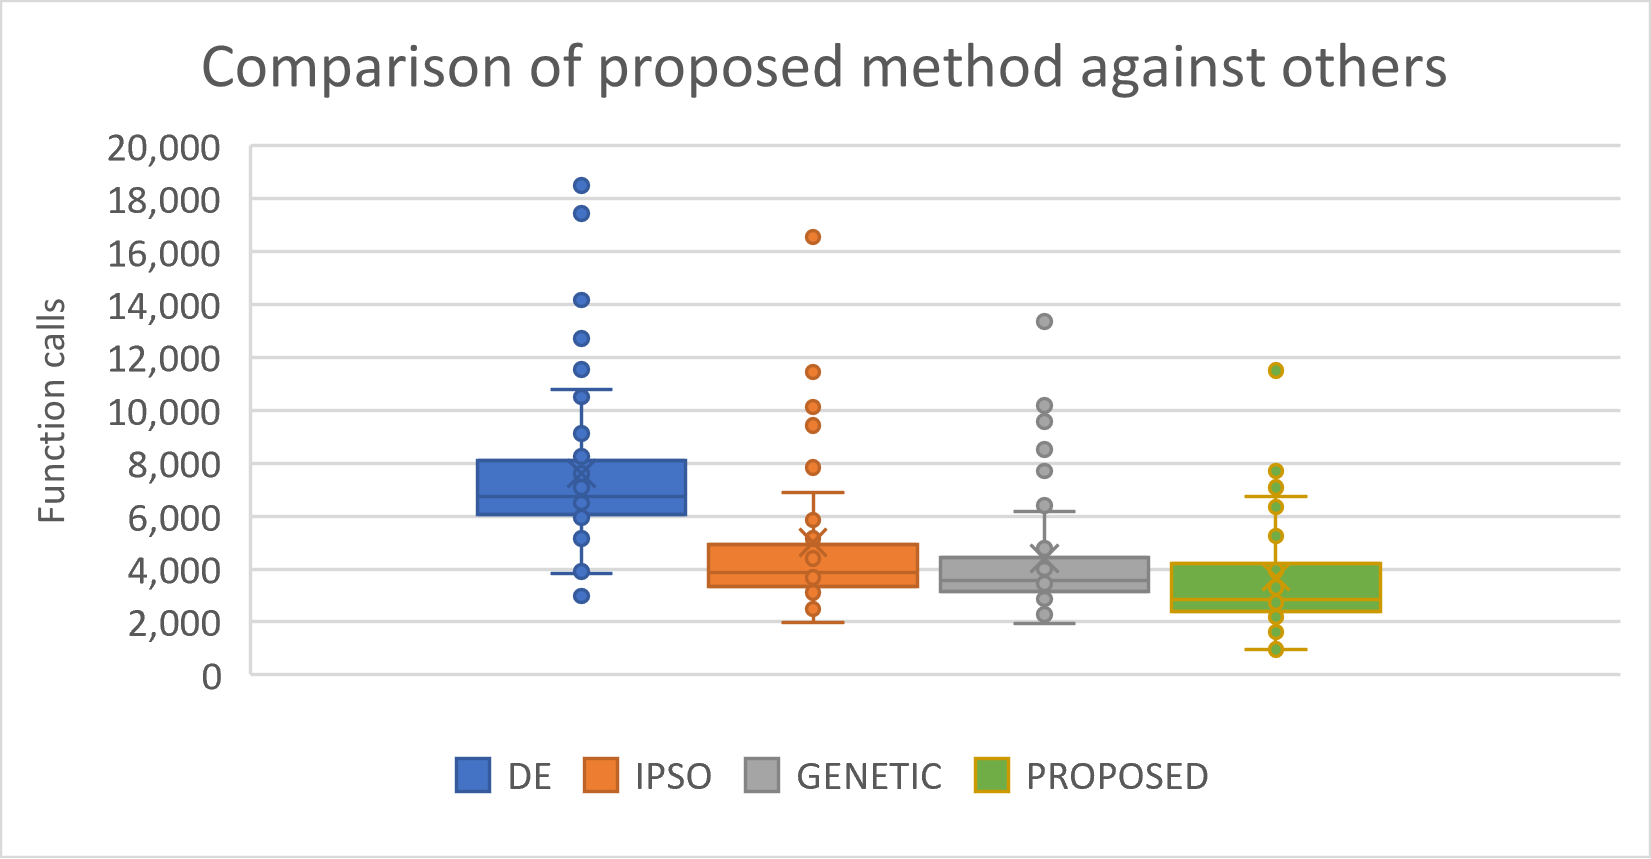
\includegraphics[scale=0.75]{img1}\caption{Comparison of function calls of proposed method against others\label{fig:proposedVSOthers}}
\end{figure}
 The proposed method seems to significantly reduce the required number
of functional calls compared to other techniques, and in many functions
this reduction can exceed 50\%. This trend is also confirmed by Figure
\ref{fig:StatProposedVSOthers}, where a statistical comparison is
presented between universal optimization methods used in the experiments.

\begin{figure}[H]
\centering{}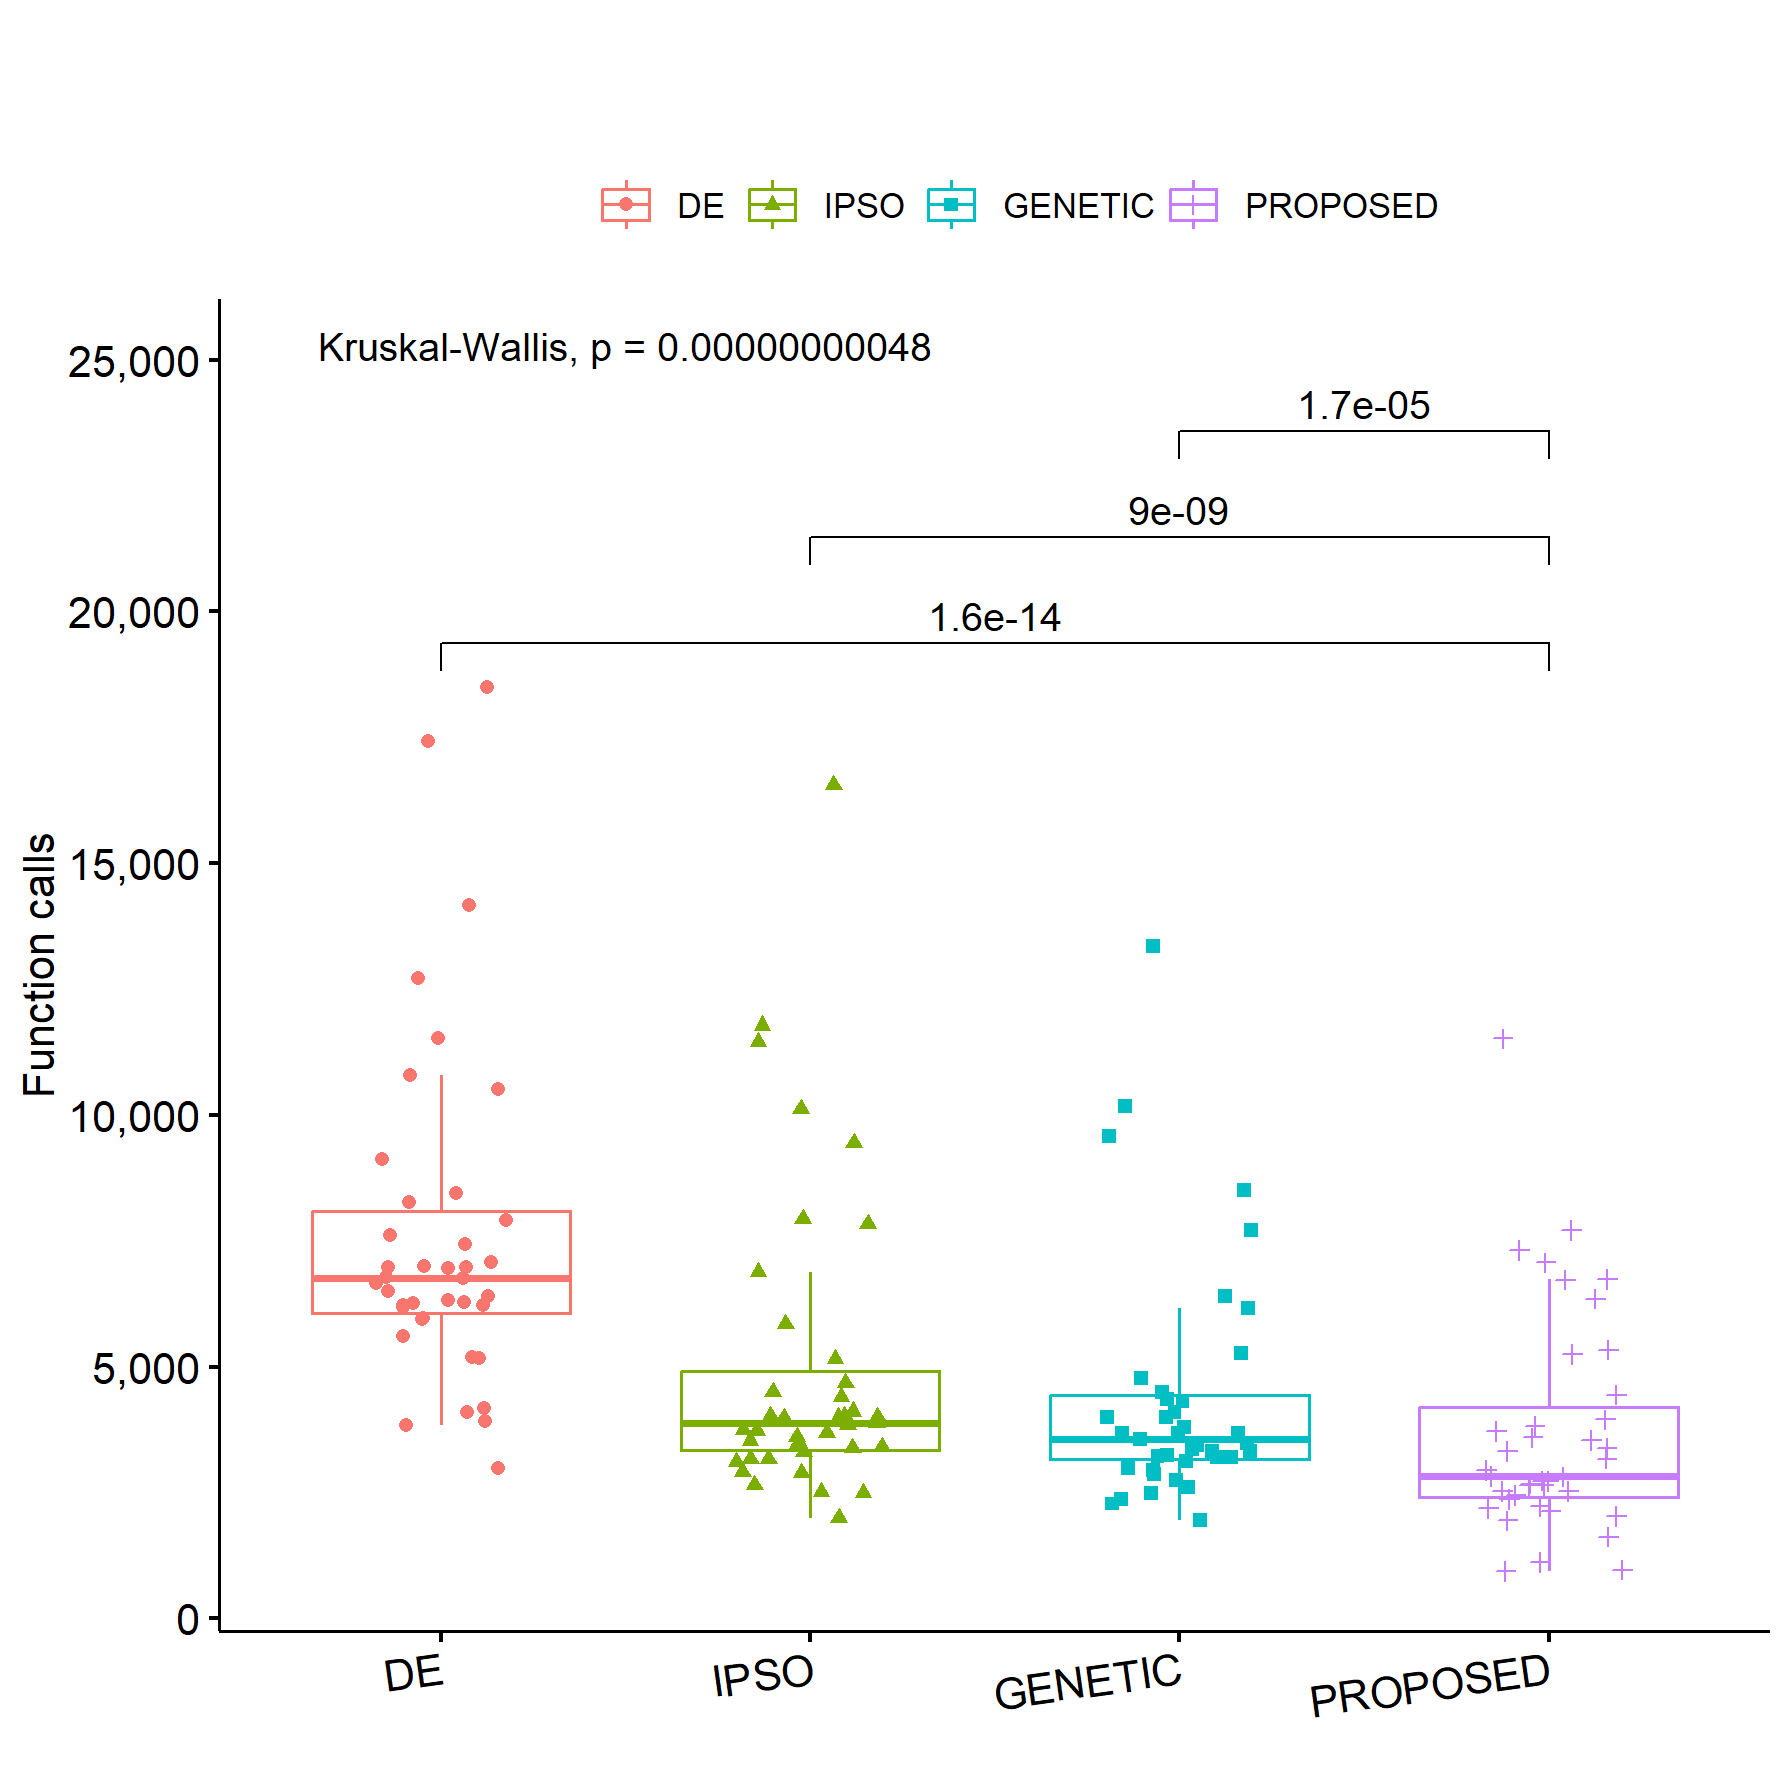
\includegraphics[scale=0.5]{MethodsStat}\caption{Statistical comparison of proposed method against others\label{fig:StatProposedVSOthers}}
\end{figure}
From the analysis presented in this Figure \ref{fig:StatProposedVSOthers},
it is abundantly clear that the proposed optimization method exhibits
a markedly superior performance when juxtaposed with the DE technique.
This superiority is evidenced by a significant reduction in computational
cost, with the proposed method requiring only 144,024 function evaluations
as opposed to the 296,929 required by DE. To substantiate this observation,
a t-test was conducted, which confirmed the presence of a statistically
significant difference, indicated by a p-value of less than 0.05.
In a comparative assessment with the iPSO method, the proposed approach
also demonstrates enhanced efficacy, achieving lower function evaluation
costs across nearly all tested functions, yielding a cost of 144,024
compared to IPSO’s 195,297. The Kruskal-Wallis test was employed to
further validate the statistical significance of this observed difference,
with results again confirming a p-value of less than 0.05. When evaluated
against the Genetic Algorithm (GENETIC), the proposed method continues
to display greater efficiency, as evidenced by a lower total cost
of 144,024 in contrast to GENETIC's 171,842. The t-test results further
reinforce this finding, highlighting a statistically significant advantage
in favor of the proposed method.

In conclusion, the proposed optimization technique demonstrates enhanced
efficiency relative to DE, IPSO, and GENETIC methodologies. The disparities
in objective function costs are not only noteworthy but are also statistically
significant, as corroborated by both parametric analysis through the
t-test and non-parametric analysis via the Kruskal-Wallis test. This
evidence collectively underscores the proposed method's superior capability
in effectively addressing the specific optimization functions evaluated
in this study.

An additional experiment was executed for the High Elliptic function,
which is defined as:
\[
f(x)=\sum_{i=1}^{n}\left(10^{6}\right)^{\frac{i-1}{n-1}}x_{i}^{2}
\]
where the parameter $n$ defines the dimension of the function. In
this particular experiment, the proposed optimization method was systematically
applied to a specific mathematical function as the dimension $n$
underwent a transition from 10 to 100. Figure \ref{fig:ELPcalls}
illustrates the performance metrics of the proposed method concerning
this function, focusing specifically on the number of function calls
made across various dimensional settings. It becomes increasingly
evident that as the dimensionality of the problem expands, the corresponding
number of function calls necessary to effectively solve the problem
also experiences a significant increase. To be more specific, when
examining the case for a dimension of 10, the algorithm requires a
total of 2,820 function calls to arrive at a solution. In stark contrast,
for a dimension of 100, the algorithm demands a staggering 23,062
function calls, which represents an increase of approximately eight
times the number of calls required at the lower dimensional level.
This notable escalation in the number of function calls as the dimensionality
of the problem grows strongly suggests that the inherent complexity
of the ELP problem scales considerably with increasing dimensionality.
Furthermore, the relationship between the number of dimensions and
the number of function calls appears to exhibit a nonlinear pattern.
This indicates that as the dimensions increase, additional computational
challenges are introduced, complicating the problem-solving process.
For instance, the transition from 10 to 20 dimensions results in more
than a doubling of the required function calls, escalating from 2,820
to 5,337. Conversely, the increase observed between 90 and 100 dimensions,
although still significant, demonstrates a somewhat smaller relative
increase, changing from 19,598 to 23,062. Additionally, Figure \ref{fig:ELPTimes}
provides a visual representation of the response times associated
with solving the ELP problem across the various dimensions, ranging
from 10 to 100, with the time measured in seconds. As anticipated,
with the increase in dimensionality, the execution time also rises
dramatically. For example, when working with 10 dimensions, the execution
time is relatively short, clocking in at only 0.224 seconds. However,
when the dimensionality is increased to 100, the execution time escalates
sharply to 32.537 seconds, marking an astonishing increase of more
than 145 times the initial time. This substantial growth in execution
time as the dimensionality of the problem increases underscores the
inherent complexity and computational demands associated with higher-dimensional
optimization problems. Moreover, the relationship between dimensions
and execution time also appears to be nonlinear, as evidenced by the
sharp increase in time observed as dimensions grow. For example, when
moving from 10 to 20 dimensions, the time required more than doubles,
rising from 0.224 seconds to 0.577 seconds. In contrast, the transition
from 90 to 100 dimensions results in an even larger jump in execution
time, from 21.897 seconds to 32.537 seconds, further illustrating
the significant challenges posed by higher-dimensional problems.
\begin{center}
\begin{figure}[H]
\begin{centering}
\subfloat[ELP: Function calls\label{fig:ELPcalls}]{\begin{centering}
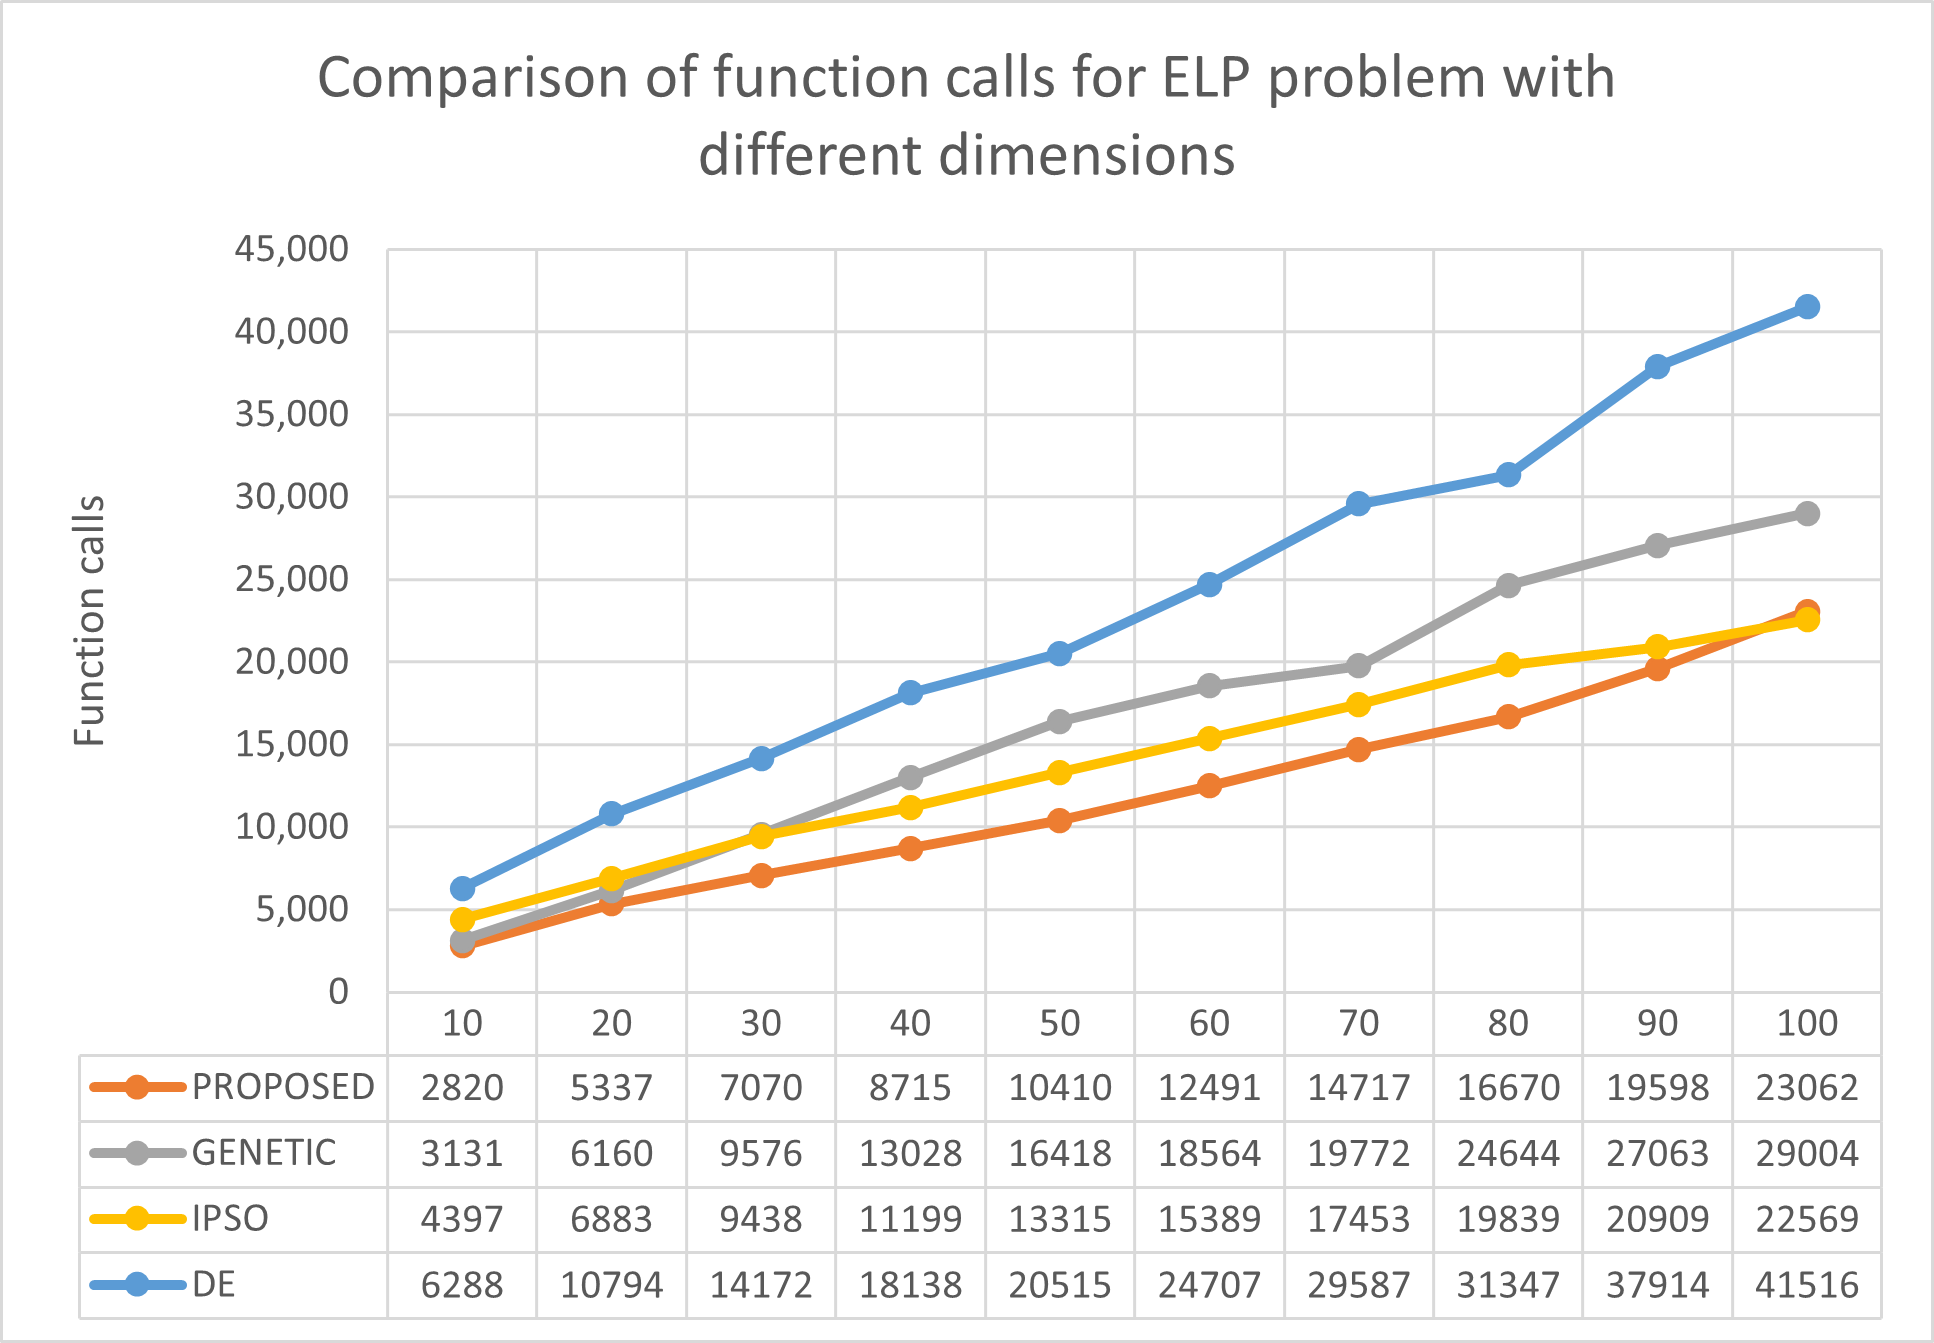
\includegraphics[scale=0.4]{img3}
\par\end{centering}
}\subfloat[ELP: Times\label{fig:ELPTimes}]{\begin{centering}
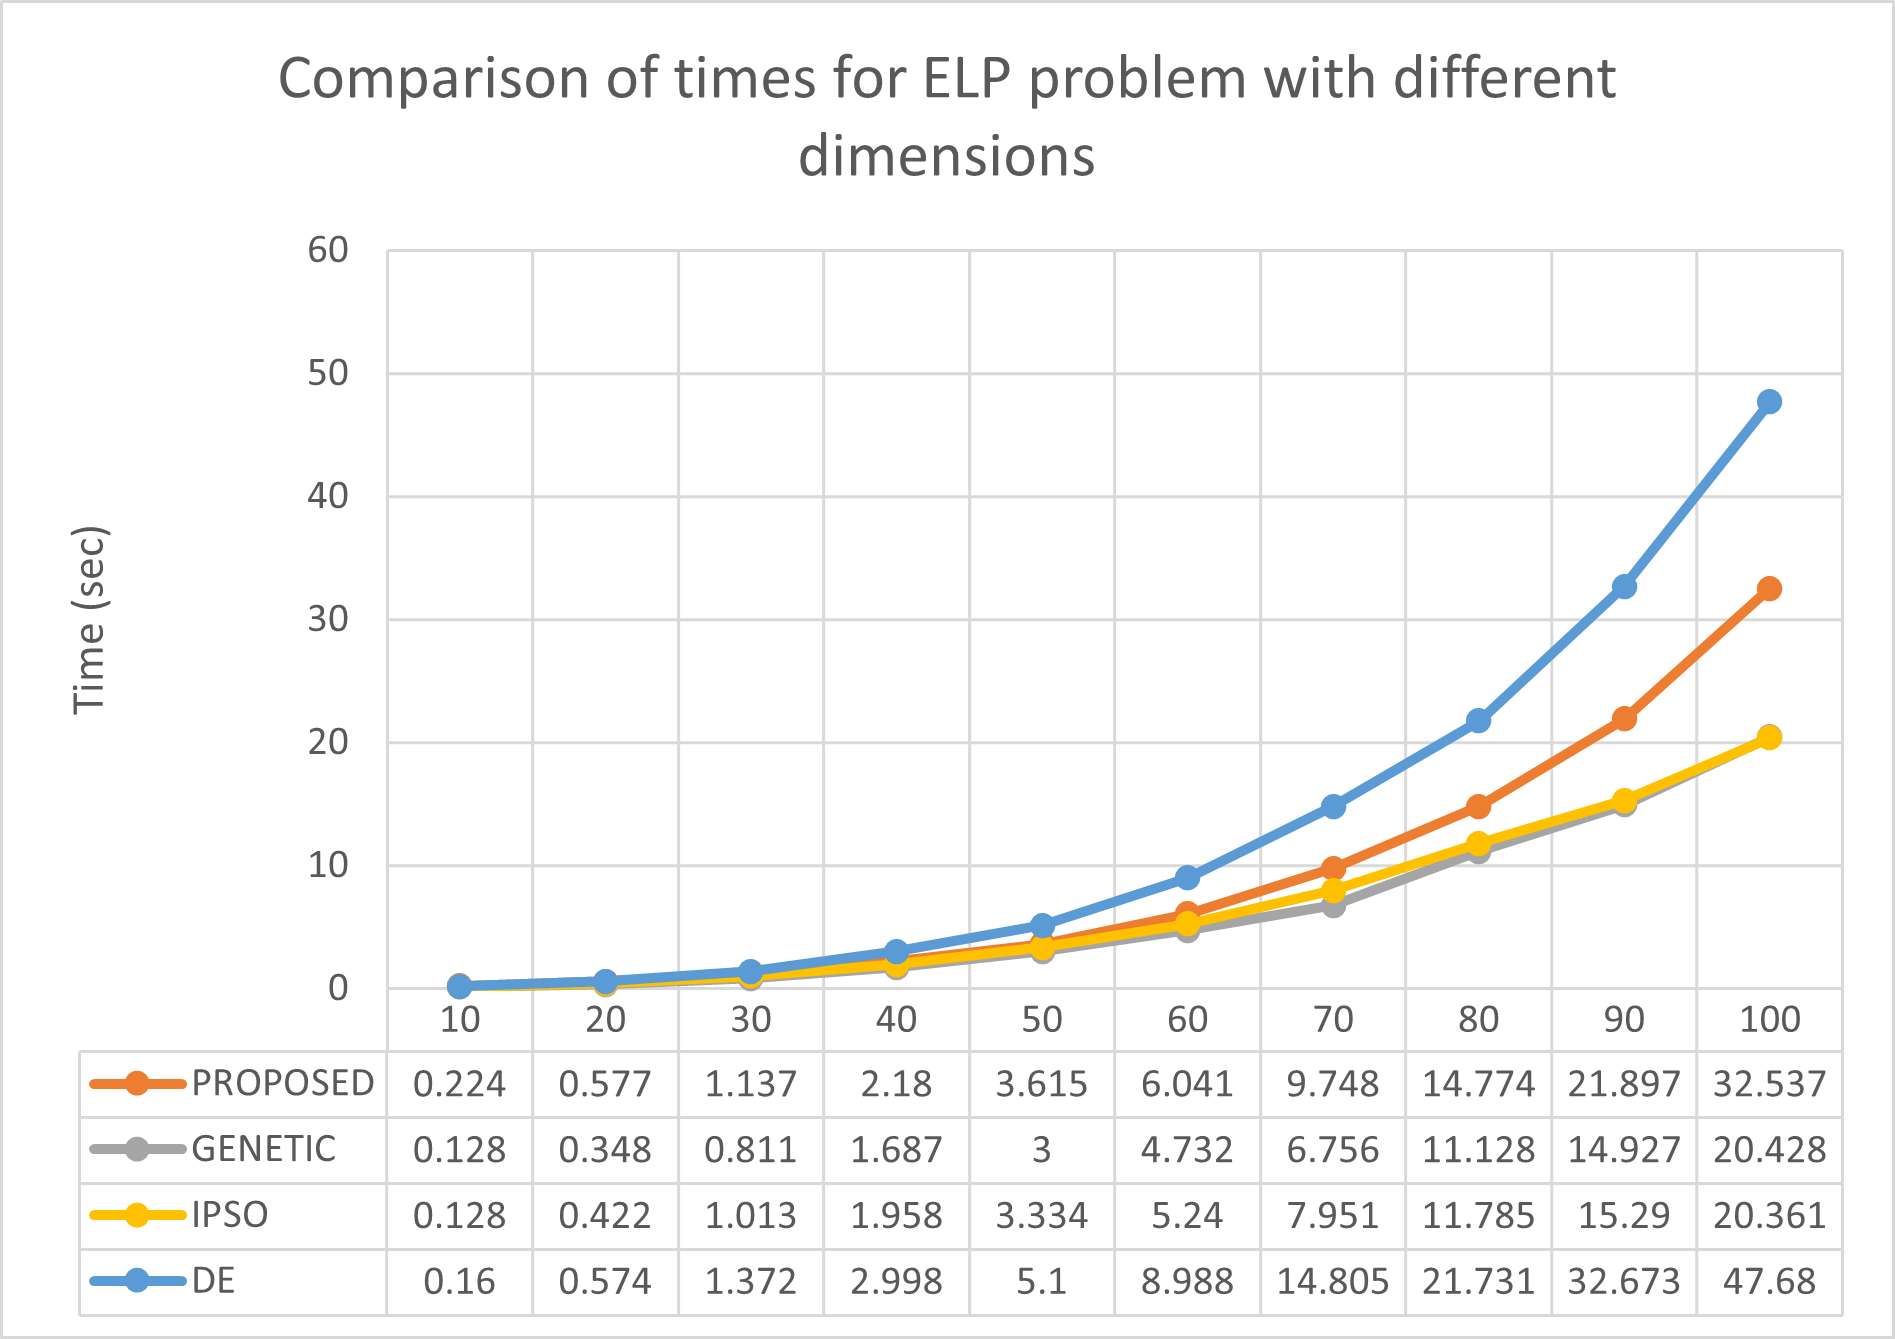
\includegraphics[scale=0.4]{img4}
\par\end{centering}
}\caption{Different variations of the ELP problem\label{fig:ELP}}
\par\end{centering}
\end{figure}
\par\end{center}

In each iteration of the algorithm, a trial point is calculated through
vector operations, similar to the process of optimization using differential
evolution. The main difference between the proposed method compared
to differential evolution lies in the fact that the samples for calculating
the trial point are selected from nearby regions of the initial distribution,
rather than being chosen randomly. However, the performance of the
two methods differs in their ability to find optimal solutions, as
shown in Figure\ref{fig:proposedVSDE}. The extraneous samples of
Figure \ref{fig:proposedVSDE} have been removed.
\begin{center}
\begin{figure}[H]
\centering{}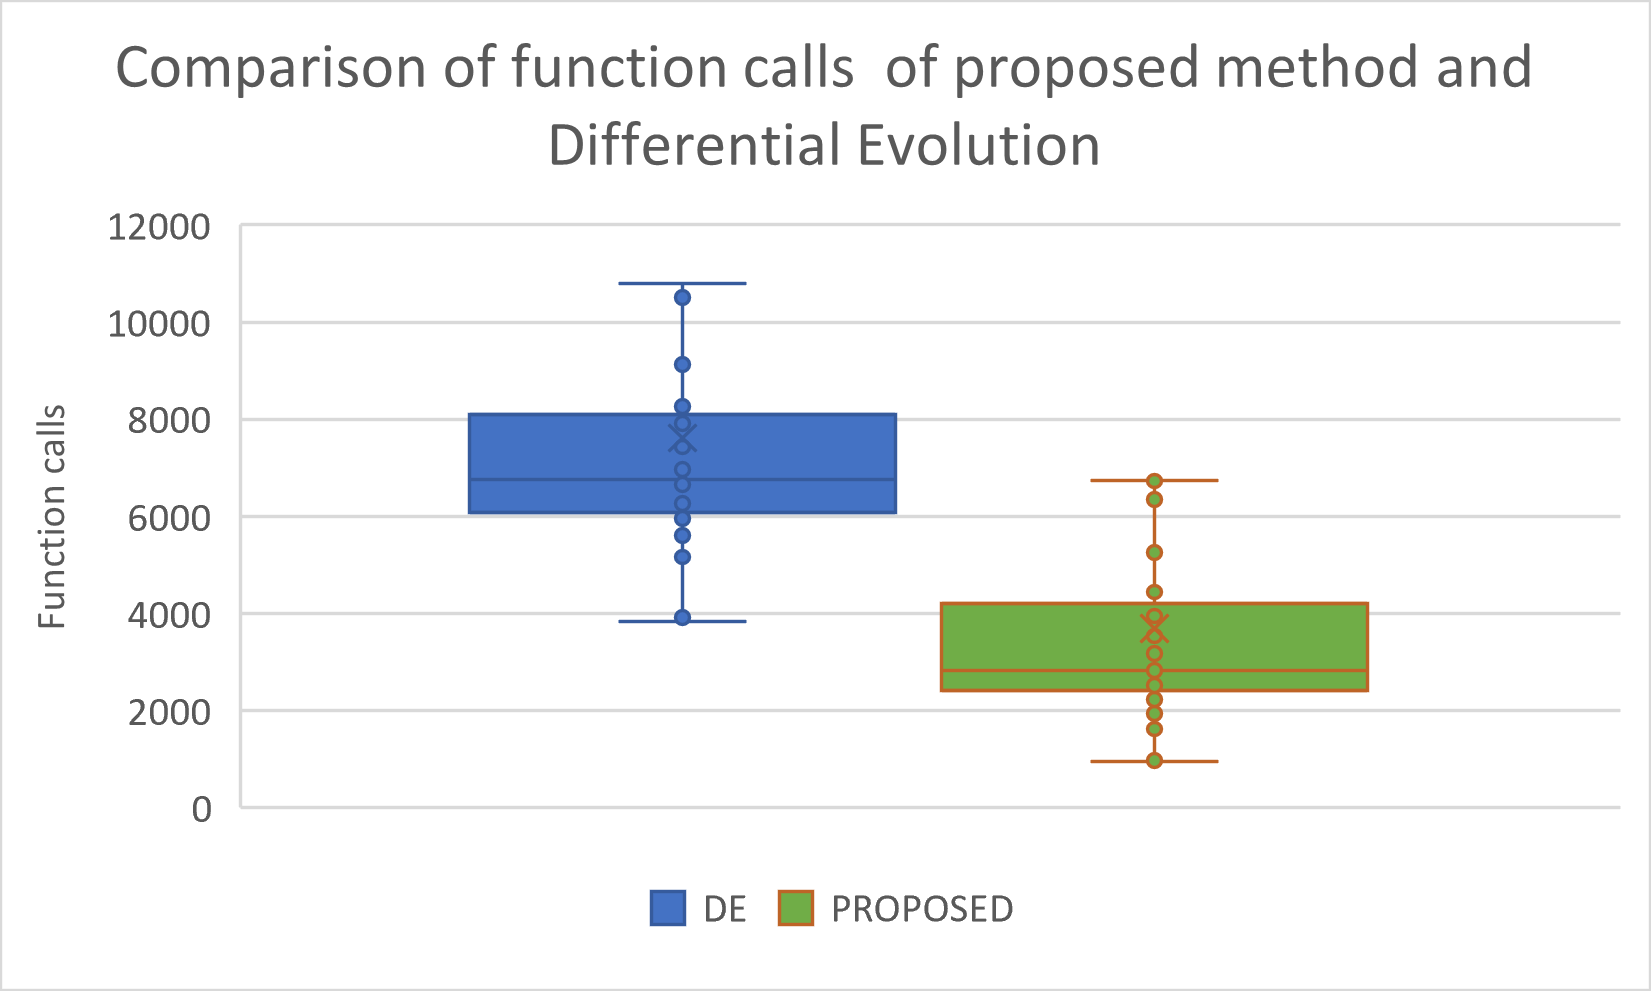
\includegraphics[scale=0.5]{img2}\caption{Comparison of proposed method against DE\label{fig:proposedVSDE}}
\end{figure}
\par\end{center}

\section{Conclusions\label{sec:Conclusions}}

An innovative global optimization method has been proposed in this
research paper, which leverages techniques derived from well-established
optimization strategies. More specifically, the new method incorporates
genetic operators from Genetic Algorithms alongside the Linear Search
method to generate candidate solutions for the given objective functions.
These candidate solutions are then combined to create new solutions
utilizing approaches inspired by the Differential Evolution method.
To validate the effectiveness of this new optimization approach, a
comprehensive series of experiments were conducted on various problems
sourced from the existing literature. Additionally, numerical comparisons
were made with recognized global optimization techniques to provide
a clear benchmark. The results indicate that the proposed optimization
method exhibits significantly superior performance when compared to
alternative methods, particularly in terms of the number of calls
made to the objective function. Fewer calls to the objective function
suggest better overall efficiency, highlighting the proposed method's
ability to achieve optimal solutions with fewer evaluations. This
efficiency is particularly critical in scenarios where each function
call is computationally expensive. Statistical analyses, including
both the t-test and the Kruskal-Wallis test, confirm that the observed
differences in the number of calls between the proposed method and
other methods are statistically significant, with a p-value of less
than 0.05. This finding not only underscores the reduced resource
consumption of the proposed method but also affirms that it delivers
reliable results with enhanced efficiency. 

In summary, the proposed method stands out in terms of efficiency
when compared to other optimization techniques, significantly decreasing
the number of objective function calls and optimizing overall computational
cost. Potential enhancements to the algorithm could involve identifying
specific samples that contribute more effectively to the discovery
of the optimal solution. Furthermore, since this method represents
a novel approach to optimization, exploring alternative termination
criteria or varying the initial sample distributions could lead to
even greater performance improvements. By refining these aspects,
the method could further bolster its efficiency and effectiveness
in solving complex optimization problems.

\vspace{6pt}


\authorcontributions{The conceptualization of the idea and the design of the methodology,
as well as the supervision of the technical aspects related to the
software, were undertaken by V.C., I.G.T., and G.K. The experiments
were conducted using various datasets, and the comparative results
were presented by V.C., G.K. and A.M.G. The statistical analysis was
carried out by V.C. The manuscript was prepared by G.K. and the other
authors. All authors have reviewed and approved the final published
version.}

\funding{No external funding was received for this research.}

\institutionalreview{Not applicable.}

\informedconsent{Not applicable. }

\institutionalreview{Not applicable.}

\acknowledgments{The experiments for this research were conducted using the high-performance
computing system installed at the Knowledge and Intelligent Computing
Laboratory, Department of Informatics and Telecommunications, University
of Ioannina, which was acquired through the project \textquotedbl Educational
Laboratory Equipment of TEI of Epirus\textquotedbl{} with MIS 5007094,
funded by the Operational Programme \textquotedbl Epirus\textquotedbl{}
2014--2020, through ERDF and national funds}

\conflictsofinterest{No conflicts of interest are declared by the authors.}

\appendixtitles{no}

\reftitle{References}
\begin{thebibliography}{999}
\bibitem{go_math1}Intriligator, M. D. (2002). Mathematical optimization
and economic theory. Society for Industrial and Applied Mathematics.

\bibitem{go_math2}Cánovas, M. J., Kruger, A., Phu, H. X., \& Théra,
M. (2020). Marco A. López, a Pioneer of Continuous Optimization in
Spain. Vietnam Journal of Mathematics, 48, 211-219.

\bibitem{go_math3}Mahmoodabadi, M. J., \& Nemati, A. R. (2016). A
novel adaptive genetic algorithm for global optimization of mathematical
test functions and real-world problems. Engineering Science and Technology,
an International Journal, 19(4), 2002-2021.

\bibitem{go_physics1}E. Iuliano, Global optimization of benchmark
aerodynamic cases using physics-based surrogate models, Aerospace
Science and Technology \textbf{67}, pp.273-286, 2017.

\bibitem{go_physics2}Q. Duan, S. Sorooshian, V. Gupta, Effective
and efficient global optimization for conceptual rainfall-runoff models,
Water Resources Research \textbf{28}, pp. 1015-1031 , 1992.

\bibitem{go_physics3}L. Yang, D. Robin, F. Sannibale, C. Steier,
W. Wan, Global optimization of an accelerator lattice using multiobjective
genetic algorithms, Nuclear Instruments and Methods in Physics Research
Section A: Accelerators, Spectrometers, Detectors and Associated Equipment
\textbf{609}, pp. 50-57, 2009.

\bibitem{go_chem1}S. Heiles, R. L. Johnston, Global optimization
of clusters using electronic structure methods, Int. J. Quantum Chem.
\textbf{113}, pp. 2091-- 2109, 2013.

\bibitem{go_chem2}W.H. Shin, J.K. Kim, D.S. Kim, C. Seok, GalaxyDock2:
Protein--ligand docking using beta-complex and global optimization,
J. Comput. Chem. \textbf{34}, pp. 2647-- 2656, 2013.

\bibitem{go_chem3}A. Liwo, J. Lee, D.R. Ripoll, J. Pillardy, H. A.
Scheraga, Protein structure prediction by global optimization of a
potential energy function, Biophysics \textbf{96}, pp. 5482-5485,
1999.

\bibitem{go_med1}Eva K. Lee, Large-Scale Optimization-Based Classification
Models in Medicine and Biology, Annals of Biomedical Engineering \textbf{35},
pp 1095-1109, 2007.

\bibitem{go_med2}Y. Cherruault, Global optimization in biology and
medicine, Mathematical and Computer Modelling \textbf{20}, pp. 119-132,
1994.

\bibitem{medicine}Houssein, E. H., Hosney, M. E., Mohamed, W. M.,
Ali, A. A., \& Younis, E. M. (2023). Fuzzy-based hunger games search
algorithm for global optimization and feature selection using medical
data. Neural Computing and Applications, 35(7), 5251-5275.

\bibitem{go_bio1}Banga, J.R. Optimization in computational systems
biology. BMC Syst. Biol. 2008, 2, 47. 

\bibitem{go_bio2}Beites, T.; Mendes, M.V. Chassis optimization as
a cornerstone for the application of synthetic biology based strategies
in microbial secondary metabolism. Front. Microbiol. 2015, 6, 159095. 

\bibitem{go_agri1}Filip, M.; Zoubek, T.; Bumbalek, R.; Cerny, P.;
Batista, C.E.; Olsan, P.; Bartos, P.; Kriz, P.; Xiao, M.; Dolan, A.;
et al. Advanced computational methods for agriculture machinery movement
optimization with applications in sugarcane production. Agriculture
2020, 10, 434

\bibitem{go_agri2}Zhang, D.; Guo, P. Integrated agriculture water
management optimization model for water saving potential analysis.
Agric. Water Manag. 2016, 170, 5--19.

\bibitem{go_econ1}Intriligator, M.D. Mathematical Optimization and
Economic Theory; SIAM: Philadelphia, PA, USA, 2002

\bibitem{go_econ2}Dixit, A.K. Optimization in Economic Theory; Oxford
University Press: Oxford, MA, USA, 1990.

\bibitem{go_determ1}Ion, I. G., Bontinck, Z., Loukrezis, D., Römer,
U., Lass, O., Ulbrich, S., ... \& De Gersem, H. (2018). Robust shape
optimization of electric devices based on deterministic optimization
methods and finite-element analysis with affine parametrization and
design elements. Electrical Engineering, 100(4), 2635-2647.

\bibitem{go_determ2}Cuevas-Velásquez, V., Sordo-Ward, A., García-Palacios,
J. H., Bianucci, P., \& Garrote, L. (2020). Probabilistic model for
real-time flood operation of a dam based on a deterministic optimization
model. Water, 12(11), 3206.

\bibitem{go_determ3}Pereyra, M., Schniter, P., Chouzenoux, E., Pesquet,
J. C., Tourneret, J. Y., Hero, A. O., \& McLaughlin, S. (2015). A
survey of stochastic simulation and optimization methods in signal
processing. IEEE Journal of Selected Topics in Signal Processing,
10(2), 224-241.

\bibitem{stohastic}Hannah, L. A. (2015). Stochastic optimization.
International Encyclopedia of the Social \& Behavioral Sciences, 2,
473-481.

\bibitem{stohastic1}Kizielewicz, B., \& Sałabun, W. (2020). A new
approach to identifying a multi-criteria decision model based on stochastic
optimization techniques. Symmetry, 12(9), 1551.

\bibitem{stohastic2}Chen, T., Sun, Y., \& Yin, W. (2021). Solving
stochastic compositional optimization is nearly as easy as solving
stochastic optimization. IEEE Transactions on Signal Processing, 69,
4937-4948.

\bibitem{interval1}M.A. Wolfe, Interval methods for global optimization,
Applied Mathematics and Computation \textbf{75}, pp. 179-206, 1996.

\bibitem{interval2}T. Csendes and D. Ratz, Subdivision Direction
Selection in Interval Methods for Global Optimization, SIAM J. Numer.
Anal. \textbf{34}, pp. 922--938, 1997. 

\bibitem{Sergeyev}Y.D. Sergeyev, D.E. Kvasov, M.S. Mukhametzhanov,
On the efficiency of nature-inspired metaheuristics in expensive global
optimization with limited budget. Sci Rep \textbf{8}, 453, 2018.

\bibitem{genetic1}D. Goldberg, Genetic Algorithms in Search, Optimization
and Machine Learning, Addison-Wesley Publishing Company, Reading,
Massachussets, 1989.

\bibitem{genetic2}Z. Michaelewicz, Genetic Algorithms + Data Structures
= Evolution Programs. Springer - Verlag, Berlin, 1996.

\bibitem{genetic3}Charilogis, V., Tsoulos, I. G., \& Stavrou, V.
N. (2023). An Intelligent Technique for Initial Distribution of Genetic
Algorithms. Axioms, 12(10), 980.

\bibitem{diffe1}R. Storn, K. Price, Differential Evolution - A Simple
and Efficient Heuristic for Global Optimization over Continuous Spaces,
Journal of Global Optimization \textbf{11}, pp. 341-359, 1997.

\bibitem{diffe2}J. Liu, J. Lampinen, A Fuzzy Adaptive Differential
Evolution Algorithm. Soft Comput \textbf{9}, pp.448--462, 2005.

\bibitem{pso_major}J. Kennedy and R. Eberhart, \textquotedbl Particle
swarm optimization,\textquotedbl{} Proceedings of ICNN'95 - International
Conference on Neural Networks, 1995, pp. 1942-1948 vol.4, doi: 10.1109/ICNN.1995.488968.

\bibitem{pso1}Riccardo Poli, James Kennedy kennedy, Tim Blackwell,
Particle swarm optimization An Overview, Swarm Intelligence \textbf{1},
pp 33-57, 2007. 

\bibitem{pso2}Ioan Cristian Trelea, The particle swarm optimization
algorithm: convergence analysis and parameter selection, Information
Processing Letters \textbf{85}, pp. 317-325, 2003.

\bibitem{aco1}M. Dorigo, M. Birattari and T. Stutzle, Ant colony
optimization, IEEE Computational Intelligence Magazine \textbf{1},
pp. 28-39, 2006.

\bibitem{aco2}K. Socha, M. Dorigo, Ant colony optimization for continuous
domains, European Journal of Operational Research 185, pp. 1155-1173,
2008.

\bibitem{fish}M. Neshat, G. Sepidnam, M. Sargolzaei, et al, Artificial
fish swarm algorithm: a survey of the state-of-the-art, hybridization,
combinatorial and indicative applications, Artif Intell Rev \textbf{42},
pp. 965--997, 2014.

\bibitem{dolphin}Tq. Wu, M. Yao, Jh. Yang, Dolphin swarm algorithm,
Frontiers Inf Technol Electronic Eng \textbf{17}, pp. 717--729, 2016. 

\bibitem{WOA}Mirjalili, S., Lewis, A.: The whale optimization algorithm.
Adv. Eng. Softw. 95, 51--67 (2016)

\bibitem{WOA1}Nasiri, J., \& Khiyabani, F. M. (2018). A whale optimization
algorithm (WOA) approach for clustering. Cogent Mathematics \& Statistics,
5(1), 1483565.

\bibitem{WOA2}Gharehchopogh, F. S., \& Gholizadeh, H. (2019). A comprehensive
survey: Whale Optimization Algorithm and its applications. Swarm and
Evolutionary Computation, 48, 1-24.

\bibitem{gpu1}Y. Zhou and Y. Tan, \textquotedbl GPU-based parallel
particle swarm optimization,\textquotedbl{} 2009 IEEE Congress on
Evolutionary Computation, pp. 1493-1500, 2009.

\bibitem{gpu2}L. Dawson and I. Stewart, \textquotedbl Improving
Ant Colony Optimization performance on the GPU using CUDA,\textquotedbl{}
2013 IEEE Congress on Evolutionary Computation, 2013, pp. 1901-1908,
doi: 10.1109/CEC.2013.6557791.

\bibitem{gpu3}Barkalov, K., Gergel, V. Parallel global optimization
on GPU. J Glob Optim 66, 3--20 (2016). 

\bibitem{holland}Holland, J.H. Genetic algorithms. Sci. Am. 1992,
267, 66--73.

\bibitem{ga_problem1}Y.H. Santana, R.M. Alonso, G.G. Nieto, L. Martens,
W. Joseph, D. Plets, Indoor genetic algorithm-based 5G network planning
using a machine learning model for path loss estimation, Appl. Sci.
\textbf{12}, 3923. 2022.

\bibitem{ga_problem2}X. Liu, D. Jiang, B. Tao, G. Jiang, Y. Sun,
J. Kong, B. Chen, Genetic algorithm-based trajectory optimization
for digital twin robots, Front. Bioeng. Biotechnol \textbf{9}, 793782,
2022.

\bibitem{ga_problem3}K. Nonoyama, Z.Liu, T. Fujiwara, M.M. Alam,
T. Nishi, Energy-efficient robot configuration and motion planning
using genetic algorithm and particle swarm optimization, Energies
\textbf{15}, 2074, 2022.

\bibitem{ga_problem4}K. Liu, B. Deng, Q. Shen, J. Yang, Y. Li, Optimization
based on genetic algorithms on energy conservation potential of a
high speed SI engine fueled with butanol--gasoline blends, Energy
Rep. \textbf{8}, pp. 69--80, 2022.

\bibitem{ga_problem5}G. Zhou, S. Zhu, S. Luo, Location optimization
of electric vehicle charging stations: Based on cost model and genetic
algorithm, Energy \textbf{247}, 123437, 2022.

\bibitem{ga_nn1}J. Arifovic, R. Gençay, Using genetic algorithms
to select architecture of a feedforward artificial neural network,
Physica A: Statistical Mechanics and its Applications \textbf{289},
pp. 574-594, 2001. 

\bibitem{ga_nn2}F. H. F. Leung, H. K. Lam, S. H. Ling, P. K. S. Tam,
Tuning of the structure and parameters of a neural network using an
improved genetic algorithm, IEEE Transactions on Neural Networks \textbf{14},
pp. 79-88, 2003.

\bibitem{de_symmetry1}Y.H. Li, J.Q. Wang, X.J. Wang, Y.L. Zhao, X.H.
Lu, D.L. Liu, Community Detection Based on Differential Evolution
Using Social Spider Optimization, Symmetry \textbf{9}, 2017.

\bibitem{de_symmetry2}W. Yang, E.M. Dilanga Siriwardane, R. Dong,
Y. Li, J. Hu, Crystal structure prediction of materials with high
symmetry using differential evolution, J. Phys.: Condens. Matter \textbf{33}
455902, 2021.

\bibitem{de_problem1}Maulik, U.; Saha, I. Automatic Fuzzy Clustering
Using Modified Differential Evolution for Image Classification. IEEE
Trans. Geosci. Remote Sens. 2010, 48, 3503--3510.

\bibitem{de_problem2}Zhang, Y.; Zhang, H.; Cai, J.; Yang, B. A Weighted
Voting Classifier Based on Differential Evolution. Abstr. Appl. Anal.
2014, 2014, 376950.

\bibitem{de_problem3}Hancer, E. Differential evolution for feature
selection: A fuzzy wrapper--filter approach. Soft Comput. 2019, 23,
5233--5248.

\bibitem{de_problem4}Vivekanandan, T.; Iyengar, N.C.S.N. Optimal
feature selection using a modified differential evolution algorithm
and its effectiveness for prediction of heart disease. Comput. Biol.
Med. 2017, 90, 125--136.

\bibitem{de_deep1}Deng, W.; Liu, H.; Xu, J.; Zhao, H.; Song, Y. An
Improved Quantum-Inspired Differential Evolution Algorithm for Deep
Belief Network. IEEE Trans. Instrum. Meas. 2020, 69, 7319--7327.

\bibitem{de_deep2}Wu, T.; Li, X.; Zhou, D.; Li, N.; Shi, J. Differential
Evolution Based Layer-Wise Weight Pruning for Compressing Deep Neural
Networks. Sensors 2021, 21, 880.

\bibitem{go_local2}H. Badem, A. Basturk, A. Caliskan, M.E. Yuksel,
A new hybrid optimization method combining artificial bee colony and
limited-memory BFGS algorithms for efficient numerical optimization,
Applied Soft Computing \textbf{70}, pp. 826-844, 2018.

\bibitem{go_local3}A.A. Nagra, F. Han, Q.H. Ling, An improved hybrid
self-inertia weight adaptive particle swarm optimization algorithm
with local search, Engineering Optimization \textbf{51}, pp. 1115-1132,
2018.

\bibitem{hybrid1}Li, S., Tan, M., Tsang, I. W., \& Kwok, J. T. Y.
(2011). A hybrid PSO-BFGS strategy for global optimization of multimodal
functions. IEEE Transactions on Systems, Man, and Cybernetics, Part
B (Cybernetics), 41(4), 1003-1014.

\bibitem{hybrid2}Andalib Sahnehsaraei, M., Mahmoodabadi, M. J., Taherkhorsandi,
M., Castillo-Villar, K. K., \& Mortazavi Yazdi, S. M. (2015). A hybrid
global optimization algorithm: particle swarm optimization in association
with a genetic algorithm. Complex System Modelling and Control Through
Intelligent Soft Computations, 45-86.

\bibitem{armijo}Armijo, L. (1966). Minimization of functions having
Lipschitz continuous first partial derivatives. Pacific Journal of
mathematics, 16(1), 1-3.

\bibitem[(2002)]{bfgs}, Convergence properties of the BFGS algoritm.
SIAM Journal on Optimization \textbf{13}, pp. 693-701, 2002.

\bibitem{charilogis}Charilogis, V.; Tsoulos, I.G. Toward an Ideal
Particle Swarm Optimizer for Multidimensional Functions. Information
2022, 13, 217. 

\bibitem{Gaviano} M. Gaviano, D.E. Ksasov, D. Lera, Y.D. Sergeyev,
Software for generation of classes of test functions with known local
and global minima for global optimization, ACM Trans. Math. Softw.
\textbf{29}, pp. 469-480, 2003.

\bibitem{Lennard} J.E. Lennard-Jones, On the Determination of Molecular
Fields, Proc. R. Soc. Lond. A \textbf{ 106}, pp. 463--477, 1924.

\bibitem{Zabinsky} Z.B. Zabinsky, D.L. Graesser, M.E. Tuttle, G.I.
Kim, Global optimization of composite laminates using improving hit
and run, In: Recent advances in global optimization, pp. 343-368,
1992.

\bibitem{Ali1}M. Montaz Ali, Charoenchai Khompatraporn, Zelda B.
Zabinsky, A Numerical Evaluation of Several Stochastic Algorithms
on Selected Continuous Global Optimization Test Problems, Journal
of Global Optimization \textbf{31}, pp 635-672, 2005. 

\bibitem{Floudas1}C.A. Floudas, P.M. Pardalos, C. Adjiman, W. Esposoto,
Z. G$\ddot{\mbox{u}}$m$\ddot{\mbox{u}}$s, S. Harding, J. Klepeis,
C. Meyer, C. Schweiger, Handbook of Test Problems in Local and Global
Optimization, Kluwer Academic Publishers, Dordrecht, 1999.

\bibitem{ipso}V. Charilogis, I.G. Tsoulos, Toward an Ideal Particle
Swarm Optimizer for Multidimensional Functions , Information \textbf{13},
217, 2022.

\bibitem{powell}Powell, M.J.D. A Tolerant Algorithm for Linearly
Constrained Optimization Calculations. Math. Program. 1989, 45, 547--566.

\end{thebibliography}

\end{document}
